%%%%%%%%%%%%%%%%%%%%%%%%%%%%%%%%%%%
%This is the LaTeX ARTICLE template for RSC journals
%Copyright The Royal Society of Chemistry 2016
%%%%%%%%%%%%%%%%%%%%%%%%%%%%%%%%%%%

\documentclass[twoside,twocolumn,9pt]{article}
\usepackage{extsizes}
\usepackage[super,sort&compress,comma]{natbib} 
\usepackage[version=3]{mhchem}
%\usepackage[left=1.5cm, right=1.5cm, top=1.785cm, bottom=2.0cm]{geometry}
\usepackage[left=1.5cm, right=1.5cm,top=0.55cm,bottom=7.0cm]{geometry}
\usepackage{balance}
\usepackage{times,mathptmx}
\usepackage{sectsty}
\usepackage{graphicx} 
\usepackage{lastpage}
\usepackage[format=plain,justification=justified,singlelinecheck=false,font={stretch=1.125,small,sf},labelfont=bf,labelsep=space]{caption}
\usepackage{float}
\usepackage{fancyhdr}
\usepackage{fnpos}
\usepackage[english]{babel}
\usepackage{array}
\usepackage{droidsans}
\usepackage{charter}
\usepackage[T1]{fontenc}
\usepackage[usenames,dvipsnames]{xcolor}
\usepackage{setspace}
\usepackage[compact]{titlesec}

\usepackage{epstopdf}%This line makes .eps figures into .pdf - please comment out if not required.

\definecolor{cream}{RGB}{222,217,201}
\newcommand{\tasadd}[1]{{\color{blue}#1}} % blue or black
\newcommand{\tasrm}[1]{\color{red}\sout{#1}} % \color{red}\sout{#1} or delete #1
\usepackage{amssymb,amsmath} % For \gtrsim

\begin{document}

\pagestyle{fancy}
\thispagestyle{plain}
\fancypagestyle{plain}{

%%%HEADER%%%
\fancyhead[C]{
\includegraphics[width=18.5cm]{head_foot/header_bar}}
\fancyhead[L]{\hspace{0cm}\vspace{1.5cm}
\includegraphics[height=30pt]{head_foot/SM}}
\fancyhead[R]{\hspace{0cm}\vspace{1.7cm}
\includegraphics[height=55pt]{head_foot/RSC_LOGO_CMYK}}
\renewcommand{\headrulewidth}{0pt}
}
%%%END OF HEADER%%%

%%%PAGE SETUP - Please do not change any commands within this section%%%
\makeFNbottom
\makeatletter
\renewcommand\LARGE{\@setfontsize\LARGE{15pt}{17}}
\renewcommand\Large{\@setfontsize\Large{12pt}{14}}
\renewcommand\large{\@setfontsize\large{10pt}{12}}
\renewcommand\footnotesize{\@setfontsize\footnotesize{7pt}{10}}
\makeatother

\renewcommand{\thefootnote}{\fnsymbol{footnote}}
\renewcommand\footnoterule{\vspace*{1pt}% 
\color{cream}\hrule width 3.5in height 0.4pt \color{black}\vspace*{5pt}} 
\setcounter{secnumdepth}{5}

\makeatletter 
\renewcommand\@biblabel[1]{#1}            
\renewcommand\@makefntext[1]% 
{\noindent\makebox[0pt][r]{\@thefnmark\,}#1}
\makeatother 
\renewcommand{\figurename}{\small{Fig.}~}
\sectionfont{\sffamily\Large}
\subsectionfont{\normalsize}
\subsubsectionfont{\bf}
\setstretch{1.125} %In particular, please do not alter this line.
\setlength{\skip\footins}{0.8cm}
\setlength{\footnotesep}{0.25cm}
\setlength{\jot}{10pt}
\titlespacing*{\section}{0pt}{4pt}{4pt}
\titlespacing*{\subsection}{0pt}{15pt}{1pt}
%%%END OF PAGE SETUP%%%

%%%FOOTER%%%
\fancyfoot{}
\fancyfoot[LO,RE]{\vspace{-7.1pt}
\includegraphics[height=9pt]{head_foot/LF}}
\fancyfoot[CO]{\vspace{-7.1pt}\hspace{13.2cm}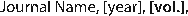
\includegraphics{head_foot/RF}}
\fancyfoot[CE]{\vspace{-7.2pt}\hspace{-14.2cm}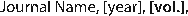
\includegraphics{head_foot/RF}}
\fancyfoot[RO]{\footnotesize{\sffamily{1--\pageref{LastPage} ~\textbar  \hspace{2pt}\thepage}}}
\fancyfoot[LE]{\footnotesize{\sffamily{\thepage~\textbar\hspace{3.45cm} 1--\pageref{LastPage}}}}
\fancyhead{}
\renewcommand{\headrulewidth}{0pt} 
\renewcommand{\footrulewidth}{0pt}
\setlength{\arrayrulewidth}{1pt}
\setlength{\columnsep}{6.5mm}
\setlength\bibsep{1pt}
%%%END OF FOOTER%%%

%%%FIGURE SETUP - please do not change any commands within this section%%%
\makeatletter 
\newlength{\figrulesep} 
\setlength{\figrulesep}{0.5\textfloatsep} 

\newcommand{\topfigrule}{\vspace*{-1pt}% 
\noindent{\color{cream}\rule[-\figrulesep]{\columnwidth}{1.5pt}} }

\newcommand{\botfigrule}{\vspace*{-2pt}% 
\noindent{\color{cream}\rule[\figrulesep]{\columnwidth}{1.5pt}} }

\newcommand{\dblfigrule}{\vspace*{-1pt}% 
\noindent{\color{cream}\rule[-\figrulesep]{\textwidth}{1.5pt}} }

\makeatother
%%%END OF FIGURE SETUP%%%

%%%TITLE, AUTHORS AND ABSTRACT%%%
\twocolumn[
  \begin{@twocolumnfalse}
\vspace{3cm}
\sffamily
\begin{tabular}{m{4.5cm} p{13.5cm} }


\includegraphics{head_foot/DOI} & \noindent\LARGE{\textbf{
Quantifying the link between local structure and cell rearrangements in the cell vertex model$^\dag$}} \\
\vspace{0.3cm} & \vspace{0.3cm} \\

 & \noindent\large{Tristan A. Sharp and Andrea J. Liu\textit{$^{a}$}} \\%Author names go here    

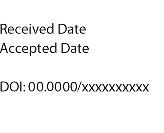
\includegraphics{head_foot/dates} & \noindent\normalsize{

% Full papers start with a brief unreferenced abstract and contain an introduction, results and discussion, experimental, and notes and references sections. A short justification statement must be included with the submission outlining why the study will appeal to the broad, interdisciplinary readership of the journal, and what fundamental issues it addresses.

Motions of cells in dense tissues can be impeded by the positions of the neighboring cells.
We use a machine learning method to investigate 
the connection between local tissue structure and cell motions called T1 transitions in the cell vertex model.
A T1 transition is a event in which cells swap neighbors, indicating a substantial cell motion.
After training, each cell in a single new snapshot can be assigned a value, softness, that strongly indicates the 
likelihood of that cell to undergo a T1 transition.
The amount of information about T1 transitions that is extracted from the local structure can be measured \emph{e.g.} in bits, giving a quantitative estimate of the degree to which these dynamics depend on structure.
We then quantify the predictive utility of local features such as shortest cell-cell contact and mean local cell shape.
} \\ 
\end{tabular}
%Any references in the abstract should be written out in full \textit{e.g.}\ [Surname \textit{et al., Journal Title}, 2000, \textbf{35}, 3523].} \\

 \end{@twocolumnfalse} \vspace{0.6cm}

  ]
%%%END OF TITLE, AUTHORS AND ABSTRACT%%%

%%%FONT SETUP - please do not change any commands within this section
\renewcommand*\rmdefault{bch}\normalfont\upshape
\rmfamily
\section*{}
\vspace{-1cm}


%%%FOOTNOTES%%%

\footnotetext{\textit{$^{a}$~Department of Physics and Astronomy, University of Pennsylvania, 209 S. 33rd St, Philadelphia, PA 19104, USA. E-mail: tsharp@sas.upenn.edu, ajliu@physics.upenn.edu}}
%\footnotetext{\textit{$^{b}$~Address, Address, Town, Country. }}

%Please use \dag to cite the ESI in the main text of the article.
%If you article does not have ESI please remove the the \dag symbol from the title and the footnotetext below.
\footnotetext{\dag~Electronic Supplementary Information (ESI) available: [details of any supplementary information available should be included here]. See DOI: 10.1039/cXsm00000x/}
%additional addresses can be cited as above using the lower-case letters, c, d, e... If all authors are from the same address, no letter is required

\footnotetext{\ddag~Additional footnotes to the title and authors can be included \textit{e.g.}\ `Present address:' or `These authors contributed equally to this work' as above using the symbols: \ddag, \textsection, and \P. Please place the appropriate symbol next to the author's name and include a \texttt{\textbackslash footnotetext} entry in the the correct place in the list.}


%%%END OF FOOTNOTES%%%

%%%MAIN TEXT%%%%
Fig 1 at a (p,T) where I have data to show saturation.

Vertex models have the remarkable feature that they capture quantitatively the rigidity transition in real epithelial tissues~\cite{bi2015density,park2015unjamming}. In such models, a cost function (called the energy) penalizes deviations of the perimeter and area of cells from preferred values. The target shape parameter $p_0$--the ratio of the preferred perimeter of a cell to the square-root of the preferred area--is a key variable that controls the mechanical response of the system. In the absence of self-propulsion or some other means of generating cell rearrangements, the system is rigid for $p_0<p_c \approx 3.81$ and fluid for values of $p_0>p_c$~\cite{bi2015density}. When cell motility $v_0$ or fluctuations in the form of a ``temperature" $T$ are added to trigger rearrangements of cells, the system fluidizes at a lower value of $p_0=p_g(T)$~\cite{bi2,SussmanPaoluzziMarchetti2018}. In the fluid phase near $p_g(T)$ the dynamics are glassy and heterogeneous~\cite{SussmanPaoluzziMarchetti2018}; some cells rearrange via T1 events, in which an edge separating two cells vanishes and an edge separating two of their neighbors appears, while other cells retain their neighbors. In this 
regime, the distance from the rigidity transition correlates strongly with the relation between fluctuations in the aspect ratio and the mean aspect ratio of cells~\cite{atia2018geometric}, underlining the connection between local cell geometry and macroscopic rigidity. Here we focus on the question of whether the propensity of a cell to participate in a T1 event can be predicted from its geometrical properties and/or the geometrical properties or positions of neighboring cells. 

Because the length of an edge that disappears during a T1 event must vanish during the event, the edge length is a predictive quantity. The T1 event marks the transition of the system from one metastable minimum to another in the energy landscape, and the initial length of the edge that disappears is correlated with the energy difference between the two metastable minima~\cite{kimHilgenfeldt2018universal}.  But the edge length is only one of many quantities that correlate with T1 events, and we show here that a linear combination of structural quantities, all of which can be extracted from video microscopy experiments on tissues, better predicts the propensity of a cell to participate in a T1 event.

In glassy liquids, the question of whether the propensity of a particle to rearrange depends on the local structural environment of a cell has been answered unequivocally in the affirmative by machine learning~\cite{cubuk2015,schoenholz2016a,cubuk2016,schoenholz2016b,cubuk2017,sussman2017,landes2019}. A similar approach has been shown to be successful in predicting the propensity of atoms in polycrystals to rearrange~\cite{sharp2018}. In all of these systems, a successful approach has been to use a support vector machine~\cite{svm} to construct a linear combination of quantities that characterize the local structural environment of a particle that correlates most strongly with rearrangements. Here we apply the same strategy to find a linear combination of structural quantities that correlates most strongly with T1 events in the thermal vertex model and self propelled voronoi model. We find that the resulting quantity, known as ``softness," is highly predictive near the glass transition and quantify the predictiveness via the information about rearrangements that it contains.

We raise the general question, how much information about some dynamical process (whether each cell will rearrange) is in a snapshot (positions but not velocities) of a complex system taken a short time before the process occurs? Then we find indications of what structural features provide the machine learning with that information.

\section{Methods}
\subsection{Simulation}

\begin{figure}[h]
\centering
  \includegraphics[height=6.5cm]{Fig1.pdf}
  \caption{\textcolor{red}{Probability distribution of softness for thermal system (a) at temperature $(T = 2.0 \cdot 10^{-3})$ and for self propelled system (b) at propulsion speed $(v_0 = 0.12)$ . The probability of rearrangement for cells  as a function of their softness
  value for thermal system (c) and self propelled  system (d).}}
  \label{CVM_softness}
\end{figure}
 
We consider the 2D Voronoi cell vertex model\cite{honda2004three,sussmanmerkelnounjam2018} with energy
\begin{equation}
\label{eq:arrhenius}
E = \sum^{N}_{i=1} \frac{1}{2}k_A (A_i - A_0)^2 + \frac{1}{2}k_L (L_i - L_0)^2
\end{equation}
where $A_i$ and $L_i$ are the area and perimeter of cell $i$, and $A_0$ and $L_0$ are target values.
The ratio $L_0/\sqrt{A_0} \equiv p_0$ defines the dimensionless target shape parameter.
 If $p_0 \lesssim 3.81$ the tissue is rigid, whereas if $p_0 \gtrsim 3.81$ the system is fluid~\cite{bi2015density}.
The associated stiffness constants $k_A$ and $k_L$ have little influence on the rigidity transition and here are taken to be $1.0$.
The initial positions of the $N$ cell centers are generated from a Poisson process within a simulation domain of area $N A_0$.
The Voronoi tessellation\cite{rycroft2009voro} of the cell centers is meant to represent the confluent tissue of cells, and energy minimization\cite{FIREminimizer} % at shape index $p_0=3.7$
creates an initial $T=0$ disordered configuration.
\textcolor{red}{
\subsection{Thermal Voronoi model}
The position of the cell centers $(r_i)$ are updated by the following equation of motion 
\begin{equation}
    \frac{dr_i}{dt}=\mu F_i + \eta_{i}
\end{equation}
where $dt$ is the integration time step, $\mu$ is the inverse friction coefficient and $F_i$ is 
the force experienced by cell i as $F_i = -\nabla E_i$. $\eta_i$ is the normally distributed random force
$(\eta_i(t)\eta_j(t^\prime)=2\mu T \delta (t-t^\prime) \delta_{ij})$ with zero mean and variance $2\mu T$. We set the inverse friction coefficient to be $\mu = 1.0$ and the integration time step to be $0.1$.}

\textcolor{red}{
\subsection{Self-Propelled Voronoi (SPV) model}
We simulate the self propelled Voronoi cell equation of motion
\begin{equation}
    \frac{dr_i}{dt}=\mu F_i + v_0 \hat{\eta_{i}}
\end{equation}
using a simple Eulerian scheme with a time step of 0.1. The force on each cell is defined by $F_i=-\nabla E_i$ and $\mu$ is the mobility (unit of inverse of frictional drag). In addition to $F_i$ each cell can also move due to its self propelled motility with constant magnitude $\frac{v_0}{\mu}$. We set $\mu = 1.0$. The polarity vector $\hat{\eta_{i}}=(cos (\theta_i), sin (\theta_i))$ is assign to each cell. We model the polarity as a unit vector that rotates randomly according to $\partial_t\theta_i=\eta_i(t)$. $\eta_i(t)$ corresponds to uncorrelated white noise, with zero mean and variance $2D_r$: $\langle \eta_i(t)\eta_j(t^\prime)\rangle =2D_r\delta(t-t^\prime)\delta_{ij}$.
}


\textcolor{red}{For a wide array of $T$ and $L_0$ values (for thermal system) and $v_0$ and $L_0$ values (for SPV system), approximately $10^5$ cells are simulated on a high-performance cluster by distributing the system into approximately $100$ independent simulations of $1024$ cells each. We did  initial thermalization at each target temperature and self propulsion speed for $10^6$ time step, the dynamics are recorded for up to $10^5$ time steps by saving the cell center positions at intervals of $t_W = 4$ or 40 time steps. (In the Voronoi vertex model used here, the entire tissue structure including cell shapes can be later recalculated from the cell center positions.) The times and locations of all T1 events are also recorded.}

%To probe the energy landscape of the system, cells are given unit mass and thermostated at temperature $T$. Each cell $i$ is subject to a force given by the 2D vector $\vec{f}_i = - \nabla_i E - \alpha \vec{v}_i + \vec{\beta}_i(t)$.

%This is achieved using a Verlet algorithm for Langevin dynamics\cite{Gronbech}. Each cell $i$ is subject to a force given by the 2D vector $\vec{f}_i = - \nabla_i E - \alpha \vec{v}_i + \vec{\beta}_i(t)$. $\vec{v}_i$ is the cell velocity and random forces $\vec{\beta}_i(t)$ correspond to uncorrelated thermal white noise, \emph{i.e.} with components having properties $\langle \beta(t) \rangle = 0$ and $\langle \beta(t) \beta(t') \rangle = 2 \alpha k_B T \delta(t-t')$. We use units where $k_B = 1$ and set the inverse friction coefficient to be $\alpha = 0.05$ and the integration time step to be $0.1$.

%For a wide array of $T$ and $L_0$ values, approximately $10^5$ cells are simulated on a high-performance cluster by distributing the system into approximately $100$ independent simulations of $1024$ cells each. After initial thermalization, the dynamics are recorded for up to $10^4$ time steps by saving the cell center positions at intervals of $t_W = 4$ or 40 time steps. (In the Voronoi vertex model used here, the entire tissue structure including cell shapes can be later recalculated from the cell center positions.) The times and locations of all T1 events are also recorded. 
%thermal is 160 time steps at ramping-down alpha, to reduce sim time

\subsection{Support Vector Machine}

To find a structural quantity that correlates strongly with T1 events, we must construct a training set for training the support vector machine, and a test set for evaluating the predictiveness of the resulting machine-learned quantity. Our training set consists of two subsets of cells--those that will soon participate in a T1 event and those that have not participated and will not participate in a T1 event for some time (these are the "rearranging" and "non-rearranging" subsets of our training set). For the rearranging subset, we begin by selecting $N_T$ T1 events randomly from the list of T1 events.  %of those that occur between time step 1000 and 4400.
For each T1 event, the cells involved are identified; these are the cells in the "rearranging" half of the training set. The "non-rearranging" subset of the training set consists of cells that do not rearrange during at least a 1600-time-step window. 

The next step in applying the support vector machine (SVM) is to quantify the local structural environment of a cell in terms of a set of structure variables. Following an approach described in earlier papers~\cite{schoenholz2016a,cubuk2017}, we calculate these quantities for the rearranging and non-rearranging subsets of cells. For each cell in the rearranging subset, we calculate the structural variables 80 timesteps before the T1 event occurs. For each cell in the non-rearranging subset, we calculate the structural variables in the center of the time window over which they do not rearrange. We have used three different sets of structural variables to construct the SVM. The first set is the standard one used in Refs.~~\cite{cubuk2015,schoenholz2016a,cubuk2016,schoenholz2016b,cubuk2017,sussman2017,sharp2018,landes2019}, introduced for machine learning applications by Behler and Parrinello~\cite{BehlerParinello2007}. The second set consists of the cell geometry variables, including those listed in Table~\ref{correlationwithS}. The full list is provided in the supplemental material. The results here are for the third set, which is the union of the two sets of structural quantities, but prediction accuracy results are quantitatively nearly identical for each of the sets, indicating that there is considerable redundancy between the two sets.

We now use a support vector machine (SVM), a generalization of linear regression. For a set of $M$ structural variables, one can construct an $M$-dimensional space with an orthogonal axis corresponding to each variable, normalized so that the variance of the distribution of each variable is unity. The local structural environment of each cell is then represented by a point in this $M$-dimensional space. The SVM constructs the $M-1$-dimensional hyperplane that best separates points belonging to the rearranging subset of the training set from those belonging to the non-rearranging subset of cells. The softness, $S$, for cell $i$ is defined as the signed distance of the point corresponding to cell $i$ (defined by the values of the structural variables for cell $i$) to the hyperplane. Cells with points on the rearranging side of the hyperplane have $S>0$ while those with points on the non-rearranging side have $S<0$.

\textcolor{red}{All training is performed at $p_0=3.75$ and $T=2.0\cdot 10^{-3}$, also  all examples data are shown at $p_0=3.75$ for both thermal and SPV system.}

\section{Results}
\subsection{Properties of softness and cross-validation accuracy}

%The softness of each cell for one instantaneous realization of the system is shown in Fig.~\ref{CVM_softness}(a). Evidently there is considerable variation in the value of softness from cell to cell. Fig.~\ref{CVM_softness}(b) shows the distribution of softnesses, $P(S)$. The distribution is skewed towards the high-$S$ side; most cells have softnesses falling within the range $-3 \le S \le 3$.  
\textcolor{red}{
The distribution of softness are shown in Fig.~\ref{CVM_softness} (a)  for thermal system at $p_0=3.75$ and $T=2\cdot 10^{-3}$  and in Fig.~\ref{CVM_softness} (b) for self propelled system at $p_0=3.75$ and $v_0=0.12$ . In Fig.~\ref{CVM_softness} (c) and Fig.~\ref{CVM_softness} (d) we show the probability of rearrangement $(P_R)$ as a function of their softness $(S)$ value for thermal system and self propelled system. From Figure Fig.~\ref{CVM_softness} (c) and Fig.~\ref{CVM_softness} (d) it is clear that $P_R$ is a strong of softness which increases by several order of magnitude.}

\textcolor{red}{
One way to assess the degree of success of softness in predicting rearrangements is to calculate the cross-validation accuracy (CV). For calculation of CV accuracy with ``10 folds," the training set is divided into 10 equal parts. Nine of the 10 parts, representing 90\% of the data in the training set, are then used to obtain a hyperplane. The prediction accuracy of the remaining 10\% of the data, called the test subset, is defined as the fraction of cells in the the test subset with $S>0$. This process is repeated 10 times in total, once for each choice of test subset; the average prediction accuracy over the 10 trials is the CV accuracy. 
We have found that CV accuracy varied from 79 \% to 92 \% for all over temperature and self propulsion speed.}

%The CV accuracy initially increases rapidly with the size of the training set $N_T$ and then levels off at around $N_T \approx 1000$ (Fig.~\ref{CVM_softness}(c)). The CV accuracy is useful for preventing over-fitting the test set and thereby over-estimating the accuracy\dag. As can be seen from Fig.~\ref{CVM_softness}(c), the CV accuracy is quite good, around 85\%. This is comparable to values obtained from fitting a wide variety of disordered solids and glassy liquids~\cite{cubuk2017}. We have found that CV accuracy varied from 79 \% to 92 \% for all over temperature and self propulsion speed.

A more physical way of assessing the success of $S$ is to calculate $P_R(S)$, the fraction of cells of a given $S$ that will later rearrange (between 40 and 80 time steps later, though the results are not sensitive to this precise window). This quantity is plotted vs $S$ for $T=2 \cdot 10^{-3}$ and $p_0=3.75$. Evidently, we find that $P_R(S)$ rises monotonically by several order of magnitude with increasing $S$, and that cells with large positive $S$ are several orders of magnitude more likely to rearrange than cells with large negative $S$. This result shows that softness does indeed predict the propensity of a cell to rearrange. Note that
$P_R(S)$ provides a more complete story than CV accuracy, which only considers the two categories of cells, rearranging or non-rearranging according to the definitions of the two subsets of the training set.
A cell would fall in neither of these categories if it participates in a T1 transition within the $\tau_W=40$ timestep time window but not at 80 time steps in the future. In contrast, $P_R(S)$ includes all types of cells.

\textcolor{red}{
The predictiveness of softness may be compared with that obtained for individual local structural quantities $(X)$. In Fig.~\ref{Qpercentile}, $P_R$ is again plotted, but $X$ is mapped to the interval [0,1] by plotting by percentile, $X(S)$. The values of $P_R$ for different percentiles are shown also for the cell's own shape parameter, $p \equiv L / \sqrt(A)$, cell neighbour which have highest shape parameter, 
$p_\text{hn}$, and the length of the shortest edge of the cell, $l_\text{min}$. For $l_\text{min}$, both the cell's own edges and those edges next to the cell are considered, since a T1 transition that eliminates any of those implies a change of neighbors.}

A quantity that yields a curve that lies on the average rearrangement rate (horizontal magenta line), would completely fail to predict rearrangements, since the cells would rearrange at the average rate irrespective of their value of that quantity. In order for the quantity to be predictive, its $P_R$ curve should be monotonic with a large deviation from the average rearrangement line. Clearly, the range of $P_R$ spanned by softness $(S)$ is higher than for any other structural quantity studied. This means that the probability of undergoing a rearrangement is more sensitive to softness. 


\begin{figure}%[h]
\centering
  \includegraphics[height=7.2cm]{Fig2.pdf}
  \caption{\textcolor{red}{Probability to rearrange vs the percentile $X$ in the thermal system of each structural quantity. $Softness$ - black solid, cell own shape parameter $(p)$ - red dash-dotted, cell neighbour which have highest shape parameter $(p_\text{hn})$ - blue dotted, $1/l_\text{min}$ - green dash. The large slope indicates that high-$S$ cells are much more likely to rearrange than low-$S$ cells. The magenta horizontal line represents the average rearrangement rate for cells.}}
  \label{Qpercentile}
\end{figure}

%\subsection{Arrhenius behaviour of probability of rearrangement for given softness }
\subsection{Quantifying information gained}

We quantify the predictive power of each structural quantity in terms of the information it contains about rearrangements. The information extracted from the structure about $P_R$ can be measured in bits.
A cell rearrangement in the thermal system is a random event with two possible outcomes - the cell will rearrange or else will not rearrange within the time window.
The Shannon entropy is $I(F) \equiv - F \text{log}_2 F - (1-F) \text{log}_2 (1-F)$ where $F$ is the probability of rearrangement.
Different cells have different probabilities to rearrange, but this information is hidden without cell-specific information such as nearby structure surrounding the cell.
Without incorporating cell-specific information, all cells must be taken to have the same probability to rearrange; in contrast, consideration of a structural feature such as softness permits cells to be distinguished to some degree by their values of $F$.

Without consideration of structure, but allowing a given system to be observed for some time to learn the average rearrangement rate, the value of $F$ for all cells can be refined as far as the system-averaged $P_R$, $\langle P_R \rangle$, the fraction of cells in the simulation that rearrange during time intervals of that duration.
With this prior knowledge, $F=\langle P_R \rangle$.
The corresponding entropy $I_\text{max} \equiv I(\langle P_R \rangle)$ is the same for all cells, and so for the whole system, $I_\text{max}$ is the maximum information that can be gained per cell, corresponding to complete certainty about whether each cell will rearrange.

Calculation of a structural quantity $Z$ represents a gain of information, and the entropy of a cell with value $Z$ becomes $e_Z \equiv I(P_R(Z))$.
The information gained is the decrease in entropy, and averaging over all cells in the system, the information gained per cell is $I_Z \equiv \sum (I_\text{max} - e_Z) /N \to \int dX (I_\text{max} - e_Z)$.


Clearly, if a quantity $Z$ is unrelated to rearrangements, cells are equally likely to rearrange for any value of $Z$, $P_R(X) = \langle P_R \rangle$, and $I_Z = 0$ --no information about rearrangements is gained by knowing $Z$.
This corresponds to the horizontal line on Fig.~\ref{Qpercentile}. Of all quantities investigated, $S$ (black solid line) deviates most from the horizontal line. Therefore, it contains the most information about rearrangements.
The information gained from each of the quantities is provided in Table 1. Note that the maximum available information is given by $I_\text{max}$ (col 3). 
No quantity gains the maximum available information; that would correspond to perfectly predicting a T1 event. However, we note that in a system with stochasticity, the aim is not to perfectly predict rearrangements. Our main goal is to identify a quantity that can be measured experimentally that predicts the propensity of a cell to undergo a T1 event. Our results show that softness accomplishes this most effectively.



\begin{table}[h]
\small
  \caption{\ Information in structural features about rearrangements (bits per cell). Information from quantity $Z$ is $I_Z \equiv I_\text{max}-e_Z$.}
  \label{tbl:example}
  \begin{tabular*}{0.48\textwidth}{@{\extracolsep{\fill}}cc|l|lllll}
    \hline
    $p_0$ & $T$ & $I_\text{max}$ & $I_S$ & $I_{l_{min}}$ & $I_p$ & $I_{\langle p \rangle_{neighs}}$ \\
    \hline
    3.75 & $10^{-3.0}$ & 0.027 & 0.0031 & 0.0034 & 0.00087 & 0.00071 \\
    3.75 & $10^{-3.5}$ & 0.0064 & 0.0012 & 0.0016 & 0.00040 & 0.00035 \\
    3.85 & $10^{-3.0}$ & 0.52 & 0.0089 & 0.0044 & 0.00044 & 0.00020 \\
    3.85 & $10^{-3.5}$ & 0.28 & 0.020 & 0.016 & 0.00031 & 0.00034  \\   
    \hline
  \end{tabular*}
\end{table}


\subsection{Information gained from softness as a function of $p_0$ and $T$}
\begin{figure}%[h]
\centering
  \includegraphics[height=9.0cm]{Phase_dia.pdf}
  %\includegraphics[height=6.2cm]{Fig3_2_PD.png}
  \caption{\textcolor{red}{Top Panel: The fraction of information extracted from the local structure (bluescale) approximately follows the decrease in the rate of T1 transitions: lines of constant $\langle P_R \rangle$ ($\langle P_R \rangle = 10^{-5}, 10^{-3.8}, 10^{-2.8}$ from left to right) show the increase in rearrangement rate with temperature for thermal system. Bottom panel: Similar plot for SPV system where lines of constant $\langle P_R \rangle$ ($\langle P_R \rangle = 10^{-4}, 10^{-3.5}, 10^{-3.0}, 10^{-2.5}$ from left to right) show the increase in rearrangement rate with propulsion speed for SPV system.}} 
  \label{phasediagram}
\end{figure}
The information gained by knowing softness, $I_S$, gives a measure of how glassy the dynamics are and depends on both the target shape parameter $p_0$ and on temperature $T$ for thermal system and on propulsion speed $v_0$ for SPV system. In supercooled liquids, softness provides no additional information about rearrangements above the onset temperature, $T_0$~\cite{schoenholz2016a}. Above $T_0$, the dynamics are those of an ordinary liquid, exhibiting exponential relaxation with a relaxation time that depends in an Arrhenius fashion on temperature. Below $T_0$, the dynamics show characteristically glassy liquid behavior, with stretched-exponential relaxation and a relaxation time that increases more rapidly with decreasing temperature than predicted by the Arrhenius relation.  In the thermal vertex model, there does not appear to be a clear onset temperature and the relaxation is sub-Arrhenius rather than super-Arrhenius as it is in supercooled liquids~\cite{SussmanPaoluzziMarchetti2018}. Nonetheless, we can ask how the fraction of information provided by softness, $I_S / I_\text{max}$, depends on $p_0$ and $T$ for thermal system and $p_0$ and $v_0$ for SPV system.
\textcolor{red}{The results are plotted in Fig.~\ref{phasediagram}.
At larger $p_0$ and $T$ for thermal system and at larger $p_0$ and $v_0$ for SPV system, the softness $S$ no longer contains information about whether T1 transitions will occur.
A contour of constant relaxation rate, $F$, is shown for comparison. The plot is remarkably similar to one obtained by Sussman, et al.~\cite{SussmanPaoluzziMarchetti2018} for thermal system and Bi, et al.~\cite{bi2} for SPV system, where the average shape parameter, $\langle p \rangle$ was plotted on a color scale in the $p_0-T$ plane for thermal system and diffusion constant $(D_{eff})$ (served as a dynamical order parameter) was plotted in the $p_0-v_0$ for SPV system . This implies that softness provides less information as $\langle p \rangle$ increases.}

% $\text{log}_{10}F=-4, -3.5, -3, -2.5$.

\subsection{Which structural variables are most important for softness?}
\textcolor{red}{
One way to determine which structural variables for softness are most important is to use recursive feature elimination~\cite{rfe}. Here, we instead look at which structural variables have the strongest correlations with $S$. We calculate Pearson correlation coefficients with softness for each of the structural variables (after normalization as discussed in the Appendix) used in SVM. The correlation coefficients range from 0.0 to 0.75, and are listed in Table~\ref{correlationwithS}.  Of all quantities calculated, the neighbor which have largest shape index is most highly correlated with softness. The cell's own shape index is essentially equally well-correlated with $S$, as is the highest shape index of the neighbor cells. 
%The length of the shortest edge of a cell, which was found to be strongly correlated with the energy difference between the metastable minima connected by the rearrangement, is somewhat less predictive. We distinguish between one of the cell's own edges, or an edge shared by two of its neighbors that is oriented radially from the cell. Both types are considered independently as well as together inTable~\ref{correlationwithS}, with only a minor difference in correlation with $S$ is found. (We use the inverse "1/length of shortest edge" for the correlation, since small values near zero may be expected to matter most.)
An alternative analysis based on the accuracy of an SVM in predicting T1's if trained only on one of these structural features found similar results.}


\begin{table}[h]
\centering
\small
  \caption{\ Pearson correlation coefficient ($C$) of local quantities with $S$ ($p=3.75, T=1.5 \cdot 10^{-3}$). Negative correlations are indicated by (-). ``Neighbors near $d=1.5$'' refers to the count of cells between distance $d-0.05$ and $d+0.05$ from the cell, \emph{i.e.} in a radial bin.}
  \label{correlationwithS}
  \begin{tabular*}{0.35\textwidth}{@{\extracolsep{\fill}}r|l}
    \hline
    $C$ & Feature \\
    \hline
%0.61     & Mean shape index of neighbors \\
%0.60     & Cell shape index \\
%0.59     & Highest neighboring shape index \\
%0.51     & Number of neighbors near d=1.4 \\
%0.46     & 1/length of shortest radial T1 edge \\
%0.42     & 1/length of shortest edge \\
%0.38     & Number of neighbors near d=1.3 \\
%0.37     & Number of neighbors near d=1.5 \\
%-0.36    & Mean area of neighbors \\
%-0.35    & Distance to nearest neighbor \\
%-0.35    & Number of neighbors near d=1.0 \\
%-0.33    & Cell area \\
%0.30     & Number of neighbors near d=0.7 \\
%-0.28    & Number of neighbors near d=1.1 \\
%0.26     & Number of neighbors near d=0.8 \\
%-0.18    & Number of neighbors near d=1.7 \\
%0.16     & Number of neighbors near d=1.2 \\
%0.15     & Number of neighbors near d=0.6 \\
%-0.14    & Highest neighboring cell area \\
%-0.13    & Lowest neighboring cell area \\
%0.06     & Number of neighbors near d=1.6 \\
%0.06     & Lowest neighboring cell perimeter \\
%0.05     & Highest neighboring cell perimeter \\
%-0.05    & Number of neighbors near d=0.9 \\
%0.04     & Mean perimeter of neighbors \\
%0.04     & Lowest neighboring shape index \\
%-0.03    & Number of neighbors \\
%0.02     & Cell perimeter \\

0.75     & Neighbor largest shape index \\
0.63     & Mean shape index of neighbors \\
0.61     & Cell own shape index \\
0.59     & Number of neighbors near d=1.5 \\
0.46     & Number of neighbors near d=1.6 \\
0.46     & Number of neighbors near d=2.5 \\
0.42     & Number of neighbors near d=2.4\\
-0.34     & Number of neighbors near d=1.8\\
-0.32     & Number of neighbors near d=2.8\\
-0.32     & Number of neighbors near d=2.9\\
0.32     & Number of neighbors near d=2.6\\
-0.28     & Number of neighbors near d=1.1\\
0.25     & Number of neighbors near d=0.8\\
0.23     & Number of neighbors near d=0.9\\
-0.22     & Number of neighbors near d=1.2\\
-0.12     & Number of neighbors near d=2.0\\
-0.07     & Number of neighbors near d=2.1\\
-0.05     & Number of neighbors near d=2.2\\
0.04    & Number of neighbors \\
    \hline
  \end{tabular*}
\end{table}


  






%\begin{equation}
%\label{eq:arrhenius}
%P_R(S) = \text{e}^{\Sigma(S)}\text{e}^{-\Delta E(S)/k_B T}  .
%\end{equation}

\subsection{Temperature and propulsion speed dependence of the softness distribution}
\textcolor{red}{
In supercooled liquids~\cite{schoenholz2016a,landes2019,cubuk2019}, the distribution $P(S)$ shifts to lower values of $S$ with decreasing temperature and the dynamics becomes slow. This reflects the super-Arrhenius increase of the relaxation time; the more strongly the mean value $\langle S \rangle$ shifts downwards with decreasing $T$, the more strongly super-Arrhenius the behavior~\cite{schoenholz2016b}. 
In the thermal vertex and self propelled voronoi model, Fig.~\ref{PS_vs_T} top panel shows that the similar distribution shifts to \emph{lower} values of $S$ with decreasing  temperature and self propulsion speed. The dynamics start to become more glassy as the system approach towards the rigid state. In bottom panel of
Fig.~\ref{PS_vs_T} we show the probability of rearrangement $P_R(S)$ as a function of cell softness value. The 
probability of rearrangement is calculated as a function of softness, that the cells which are rearranging at a given time.  $P_R(S)$ is plotted at different temperature $(T)$ for thermal system and at different self propulsion speed $v_0$ for SPV system. We find that $P_R(S)$ increases by several order of magnitude at different temperature and self propulsion speed indicates that it is a strong function of softness.}

%Nevertheless, the inset shows that for each value of $S$, $P_R(S)$ decreases with decreasing $T$, as expected--there are fewer rearrangements at low temperatures. These two opposing factors--the decrease of $P_R(S)$ with $T$ and the upwards shift of $P(S)$ with $T$--are consistent with  the sub-Arrhenius temperature-dependence of the relaxation time observed previously~\cite{SussmanPaoluzziMarchetti2018}. The results are consistent with an increase in effective rearrangement energy barriers with temperature due to the change of structure.


\begin{figure}[h]
\centering
  \includegraphics[height=6.4cm]{Allfig.pdf}
  \caption{\textcolor{red}{Top Panel: The distribution of softness for thermal system  as temperature $(T)$ rises and for SPV system as propulsion speed $(v_0)$ rises. Bottom Panel: The probability of rearrangement $P_R(S)$ for cells as a function of their softness value for thermal system at different temperature and for self propelled system at different self propulsion speed.}}
  \label{PS_vs_T}
\end{figure}
\textcolor{red}{
\subsection{Arrhenius behaviour of $P_R(S)$}
In Fig.~\ref{Arrhenius} top panel we have shown the $P_R(S)$ as a function of $\frac{1}{T}$ for particular softness value.
The cell for particular softness value rearranges in arrhenius way, $P_R(S) = P_0 \exp(-\frac{\Delta E(S)}{T})$, where energy barrier $\Delta E(S)$ required for activation depends on softness value. For the SPV model we define an effective temperature $T_{eff}=\frac{v_0^2}{2\mu D_r}$ \cite{PhysRevLett.108.235702} that gives an energy to trigger rearrangement of cells. However, the effective temperature mapping will be ample when rotational diffusion constant $D_r \to \infty$ for SPV system or the cells behave like Brownian particles.
In bottom panel of  Fig.~\ref{Arrhenius} we show that energy scale for thermal and SPV systems linearly depends on softness. This results are consistent with the prediction that at low temperature $(T)$ or low self propulsion speed harder region cells are fixed at their position with higher energy barrier whereas the softer regions are not.
The above observation supports the glassy behaviour (e.g. dynamics heterogeneity) in dense biological tissue.
\begin{figure}[h]
\centering
\hskip -0.2in
  \includegraphics[height=8cm]{Arrhenius_new.pdf}
  \caption{\textcolor{red}{Top Panel: $P_R(S)$ as a function of  $1/T$ for different softness values ranges from $S \sim -2$ (black) to $S \sim 2$ (magenta) for thermal system (top left). Similar plot for SPV system, where S ranges from $S \sim -2$ (black) to $S \sim 3$ (blue) (right panel). $T_{eff}$ is the effective temperature for SPV system (see text).}}
  \label{Arrhenius}
\end{figure}
}
% Stephan Koehler mentions possibly phop is more important when T1s can be reversed, which i said could be in stasis, and he thought would be at higher temperatures
\section{Discussion}
We have shown that local structure suffices to obtain a quantity, softness, that contains a considerable fraction of the maximum possible information on rearrangements. It is quite possible that improvements to the machine learning analysis (e.g. a further increase in the training set size or alternatives to the SVM) may be able to raise the information gained by a few percent. The information gained is strongly correlated with the average shape parameter $\langle p \rangle$, suggesting that $\langle p \rangle$ provides a good estimate of where in the $p_0-T$ phase diagram one might expect to find glassy dynamics. In particular, if $\langle p \rangle$ grows too large (if one is too far away from the rigid regime), local structure provides little information about rearrangements. 
In glassy systems, the lowest-frequency modes are quasilocalized; this reflects the physics that the corresponding rearrangements are localized. Sussman, et al.~\cite{SussmanPaoluzziMarchetti2018} found that by contrast the lowest-frequency vibrational modes of the 
Voronoi vertex model are spatially \emph{extended}, suggesting that the rearrangements are extended. If that is the case, it is very surprising that local structure succeeds in predicting rearrangements so well. More work in the future is required to determine whether rearrangements are indeed extended, but we note that even extended rearrangements can be broken down into a set of localized T1 events, so the ability to predict a single T1 event may suffice to predict extended rearrangements. \tasadd{[This will require dis-entangling ``rearrangement'' which could be defined as a Voronoi cell neighbor change (essentially a T1), with the associated motions of neighboring cells (contributing to the vibrational mode). I see large phop values are co-located with T1s but perhaps some smaller motions linked to the T1 are delocalized. Rearrangements won't be multiple T1s though, in my view.]}  

Our results  indicate the regime of shape parameter in which softness might be expected to be useful in epithelial tissues, and show that softness can be calculated using structural quantities that are easily obtained by video microscopy on tissues. A complication of real tissues is that cells proliferate, generating rearrangements that have a very different origin from those due to cell motility. This will require dividing the system into three subsets, cells that rearrange due to proliferation, cells that rearrange for other reasons (our current rearranging subset) and those that are stationary. Such an analysis could prove quite fruitful for real tissues.

%Anomalous result that low frequency vibrational modes are long range (so is local structure all that's important?)
%Result that energy barriers appear to rise with temperature.

For the reference section, the style file \texttt{rsc.bst} can be used to generate the correct reference style.

\section{Supplemental}

We use two sets of structure functions to quantify the local environment around each cell for input to the support vector machine. The first sets are those that we commonly use~\cite{BehlerParinello2007} that depend directly on the configuration of cell centers. We augment these  with a second data set that depends directly on the cell shapes, given by the Voronoi tessellation.

Comprising the first set, each radial structure function $R_{i\alpha}$ indicates the number of neighbors at a particular distance from the cell $i$. 
%Comprising the second set, each angular structure function $A_{i\beta}$ encodes more complicated structure using functions of angles and perimeters of triangles that can be formed with cell $i$ and pairs of its neighboring cells. These two types are given by:

\begin{equation*}
R_{i\alpha} = \sum_j \text{exp}(-(d_{ij} - \mu_{\alpha})^2/(2\sigma_0^2))
\text{,\hspace{5mm}}
\end{equation*}
%\begin{equation*}
%A_{i\beta} = \sum_{j,k} 
%%2^{1-\zeta_{\beta}} 
%(1+\lambda_{\beta} cos \theta_{ijk})^{\zeta_\beta}
%f_{ij}f_{jk}f_{ki}
%\text{,\hspace{5mm}}
%\end{equation*}
%\begin{equation*}
%f_{ij} =
%\text{exp}(-\eta_{\beta} d^2_{ij})
%\text{cos}(\pi d^2_{ij}/d_0+1)
%\text{.}
%\end{equation*}


The vector from the position of cell $i$ to the position of cell $j$ has length $d_{ij}$. 
% and it forms an angle $\theta_{ijk}$ with the vector from cell $i$ to cell $k$. 
We include 24 radial functions. % and 54 angular functions.
We use $\sigma_0=0.1$ and $\mu_\alpha = 0.7,0.8,...,2.9,3.0$ corresponding to $\alpha = \{ 0,1 \ldots 13,14,15 \ldots 22,23 \}$;
%$\eta_{\beta} = e^{-2\beta}$ for $\beta = \{ 0,1, \ldots 53 \}$;
%$\zeta_{\beta} = 0.1,0.2,...2.6,2.7,0.1,0.2,...2.6,2.7$ for $\beta = \{ 0,1, \ldots 25,26,27,28 \ldots 52,53 \}$.
%The sums include neighboring cells of $i$ out to $d_0=4.2$, a cutoff distance.

%In the third set, the following 34 values are included for each cell $i$: the number of Voronoi edges of cell $i$, then $1/L_j$ for $j=0...7$, $1/L_k$ for $k=0...7$, $1/L_l$ for $l=0...7$, the shape index $p$, and $p_j$ for $j=0...7$.
%$L_j$ is the $j-th$ shortest edge of cell $i$ (or $1/L_j=0$ if cell $i$ has less than $j$ edges).
%$L_k$ is the $k-th$ shortest edge of all edges \emph{not} belonging to cell $i$ but sharing a vertex with cell $i$ (or or $1/L_k=0$ if the cell has less than $k$ edges). The disappearance of one of these ``radial edges'' indicates that cell $i$ has connected to a new neighbor as part of a T1 transition.
%$L_l$ is the $l-th$ shortest edge of all edges that share a vertex with cell $i$, and thus is a combination of the two previous lists, sorted together.
%Finally, $p_j$ is the shape index of the Voronoi neighbor with the $j-th$ smallest shape index (or zero if cell $i$ has less than $j$ Voronoi neighbors).
%With these 34 Voronoi-dependent values, in total we consider $M=112$ structure functions. 
\textcolor{red}{
In the second set, the following 10 values are included for each cell $i$: the number of Voronoi edges of cell $i$, then the cell own shape index $p$, and $p_j$ for $j=0...7$.
Finally, $p_j$ is the shape index of the Voronoi neighbor with the $j-th$ smallest shape index (or zero if cell $i$ has less than $j$ Voronoi neighbors).
With these 10 Voronoi-dependent values, in total we consider $M=34$ structure functions. }
\textcolor{red}{
\section{Binary SPV model}
\begin{figure*}%[h]
%\centering
\begin{center}
%\hskip -0.2in
  \includegraphics[height=15cm]{SI_binary.pdf}
  \caption{\textcolor{red}{Top left Panel: $P_R(S)$ as a function of softness for different self propulsion speed $v_0$. Top right Panel: $P_R(S)$ as a function of  $1/T_{eff}$ for different softness values ranges from $S \sim -2$ (black) to $S \sim 2$ (magenta) for binary SPV system. Bottom left panel: Energy barrier vs softness. Bottom right panel: The fraction of information extracted from the local structure (blue scale) approximately follows the decrease in the rate of T1 transitions: lines of constant $\langle P_R \rangle$ ($\langle P_R \rangle = 10^{-4}, 10^{-3.5}, 10^{-3.0}, 10^{-2.5}$ from left to right) show the increase in rearrangement rate with propulsion speed for binary SPV system.}}
  \label{SI}
  \end{center}
\end{figure*}
In the main text we discussed monodisperse Voronoi model. However, for particular model parameter monodisperse system have a tendency to crystallization by reaching hexagonal ground state. Therefore 
we do the similar analysis for bidisperse self propelled voronoi model and present all the data for comparison.
In top left panel of Fig.~\ref{SI} we plot the $P_R(S)$ as a function of softness for different self propulsion speed.
It is clear for binary SPV model $P_R(S)$ is also a very strong function of softness which increase by several order of magnitude with increasing softness like monodisperse system. Top right panel we show the $P_R(S)$ as a function of $\frac{1}{T_{eff}}$, where $T_{eff}=\frac{v_0^2}{2\mu D_r}$ is the effective temperature for SPV system. We observe that similar arrhenius behaviour of probability of rearrangement for a given softness. From the arrhenius behaviour of $P_R(S)$ one can measure the energy barrier $\Delta E (S)$ as a function of softness. In bottom left panel of Fig.~\ref{SI} we show the energy barrier linearly depends on softness. In bottom right panel of Fig.~\ref{SI} we also plot the phase diagram showing the fraction of information provided by softness in $p_0$ and $v_0$ plane for binary SPV system.  
}
%IT I will show results for g(r mono and bidisperse)
%TAS WILL DELETE: This paper raises the question, how much information about some dynamical process (whether each cell will rearrange) is in a snapshot (positions but not velocities) taken a short time before the process occurs?
%The fundamental nature of the question motivates seeking the most general answer, eg one that does not depend on viewing window selected ($t_W=4$ is used here).
%Such an answer can be found using these simulations.

%We find that the information $I_S$ is largely insensitive to how long the ``short time'' is between the snapshot and the time of the prediction. This is because most cells vibrate around a static position for a long time before rearranging, at the temperatures focused on here.
%On the other hand, the choice of $t_W$ matters; note that $P_R$ is approximately proportional to the viewing interval, $t_W$, and therefore $I_S$ also depends on $t_W$.
%(Specifically $P_R \propto t_W$ since $t_W$ is short compared to the time for a particle to rearrange twice and short compared to any other relevant time scale such as system aging.) 
%It might be useful to report a quantity independent of $t_W$, such as $I'_S$, the ``information gained per time $t_W$''.
%Indeed, if we use a very small $t_W$ so that $P_R$ is sufficiently small, $I_S$ is precisely proportional to $t_W$, and in this limit we can find $I'_S$ by taking the ratio $I_S/t_W$. 
%Therefore, using these simulations and looking for rearrangements in a very small time interval $t_W$ would yield this result.
%However, in practice, $t_W$ must be very small ($I'_S$ is constant with $t_W$ for a very small range) so it is impractical here to get a precise estimate of $I'_S$. 
%On the other hand, the values of $I_S$ reported here, divided by $t_W$ are not very different from the values of $I'_S$: for values used here ($t_W=4$), $P_R(S)$ can often be $10^{-2}$ where $I_S/t_W$ is a 25\% underestimate of $I'_S$.


%p-dependence of softness.
%temperature dep of softness.
%compare diff temps at same PE??
%diff defs of rearrangements = phop. 
%Voro SFs do not improve things. 
%heterogeneity and retrain and how does it do?
%scatter plots S vs other things.
%most and least soft structures.
%more delaywindow/prediction/lead-time for rearrangement?

%%%END OF MAIN TEXT%%%

%The \balance command can be used to balance the columns on the final page if desired. It should be placed anywhere within the first column of the last page.

\balance

%If notes are included in your references you can change the title from 'References' to 'Notes and references' using the following command:
%\renewcommand\refname{Notes and references}

%%%REFERENCES%%%
\bibliography{rsc} %You need to replace "rsc" on this line with the name of your .bib file
\bibliographystyle{rsc} %the RSC's .bst file

\end{document}
